%!TEX root = ../Thesis.tex
\chapter{Hub connectivity and gene expression in \textit{C.elegans}}
\label{appendixA}

\fancyhead[R]{\textit{Appendix A:~Hub connectivity and gene expression in \textit{C.elegans}}}

\section{Expression annotations at WormBase}
\label{app:AppendixCh2_1}

Neuronal gene expression is measured as a binary indicator on WormBase \citep{Harris2010}, based on curated data collated
from many individual experiments. Expression annotations are made either ‘directly’ to individual neurons (when
an experiment indicates expression in an individual neuron), or ‘indirectly’ to broader classes of neurons like
‘interneuron’ or ‘head’ (meaning that some members of that class exhibit expression of that gene). In order to
maintain specificity of annotations, we only analysed ‘direct' annotations here.
Annotations of gene G to neuron Y are also made with varying levels of certainty:
\begin{itemize}
\item ‘certain’: G was observed to be expressed in Y,
\item ‘enriched’: G has been found to be enriched in a certain dataset through microarray, RNAseq or
proteomic analysis,
\item ‘partial’: G was observed to be expressed in some cells of a group of neurons that include Y,
\item ‘blank’: data prior to 2005, or
\item ‘uncertain’: G was sometimes observed to be expressed in Y, or G was observed to be expressed in a cell
that could be Y.
\end{itemize}

To avoid including false positives, our analysis excluded annotations labeled as ‘uncertain’.

\section{Sensitivity of correlated gene expression measures}
\label{app:AppendixCh2_2}
Measures of correlation between binary vectors can be biased by the relative proportion of ones
between two vectors. For data analysed here, data annotated to individual neurons comes from between $3$ to
$138$ expressed genes (corresponding to $0.3\%$ to $14.6\%$ of all $948$ genes considered). To ensure that our measure of correlated gene expression (CGE) is not biased by such differences in the relative proportions of expression annotations, we conducted a sensitivity analysis in which we compared the $r_\phi$ metric, Eq. \ref{eq:rphi}, with alternative
methods for quantifying correlations between binary vectors: the Jaccard index, $n_{11}/(n_{10}+n_{01}+n_{11})$, Yule's Q
coefficient, $(n_{00}n_{11}-n_{01}n_{10})/(n_{00}n_{11}+n_{01}n_{10})$, and the $\chi{^2}$, index, $N(n_{00}n_{11}-n_{01}n_{10})/(n_{0\bullet}n_{1\bullet}-n_{\bullet1}n_{\bullet0})$ \citep{Kaufman2006}, where $n_{xy}$ counts
the number of observations of each of the four binary pairwise possibilities: $n_{00}$, $n_{01}$, $n_{10}$, and $n_{11}$ (as outlined in
the main text), and the $\bullet$ symbol sums across a given variable (e.g., $n_{\bullet}= n_{00} + n_{10})$.
To evaluate bias in each CGE measure to the proportion of annotations in each expression vector, we
generated random binary vectors of length 948 containing different proportions of 1s seen in our data, ranging
from the minimum, 1, to the maximum, 150. For all pairwise combinations of proportions, we computed the CGE
measure, taking an average across $1 000$ permutations, and then recorded the resulting mean correlation value,
as plotted in Figure \ref{fig:Ch2S2_Fig}. Because all vectors are independent random binary strings, any systematic dependence of
mean CGE with annotation proportion indicates bias. The mean square contingency coefficient, (Figure \ref{fig:Ch2S2_Fig}A) and
our own novel CGE matching index, $p_{match}$ show no systematic dependence on the proportion of ones in
each vector (varying randomly within ≈ $10^{-3}$ and ≈ $0.5$ respectively). However, Yule's Q shows a negative bias for
small annotation proportions (Figure \ref{fig:Ch2S2_Fig}B) and the Jaccard index shows a strong positive bias across the full range (Figure \ref{fig:Ch2S2_Fig}C). Based on these numerical experiments, we selected mean square contingency coefficient, $r_\phi$, here, to
ensure that changes in CGE were due to matching expression patterns and not simply driven by differences in the
number of gene annotations between neurons.


\section{Correlated gene expression matching index}
\label{app:AppendixCh2_3}

Existing measures of binary correlation (described below) are symmetric between ‘0’ and ‘1’ and thus do not directly distinguish between the biologically relevant case of genes being expressed together from the case in which neither gene is expressed. We thus developed a measure of the probability, $P(m)$, that two binary strings will contain m ‘positive matches’ (i.e., m genes are expressed in both neurons), which can be computed as:


\begin{eqnarray}
	\label{eq:S3}
     P(m) = \binom{n_{2}}{m}\binom{N-n_{2}}{n_{1}-m}/\binom{N}{n_{1}},
\end{eqnarray}

for two binary expression vectors, $x_{i}$, $y_{i}$, of length N containing $n_{1}$ and $n_{2}$ 1s, respectively ($n_{1} \leq n_{2}$), with m matches ($n_{11}$). Our index, $p_{match}$, is approximately equal to the probability of obtaining as many or fewer matches than observed (weighting the probability of the observed number of matches at 0.5 for symmetry), computed as:

\begin{eqnarray}
	\label{eq:S4}
     p_{match} = \sum_{x=0}^{m-1}P(x)=P(m)/2,
\end{eqnarray}

for m positive matches.
	We verified that this index yields qualitatively similar results to the mean square contingency coefficient, $r_\phi$, (Figure \ref{fig:Ch2S3_Fig}), validating our related positive match method for scoring individual genes [as an approximately single-gene contribution to the probability score computed in Eq. \ref{eq:CBinomialProbability}].
Given the qualitative similarity of this measure to $r_\phi$, we chose to focus on $r_\phi$ throughout this work due to its ease of interpretability as a correlation coefficient ranging from -1 to 1.

\begin{figure}[h!]
  \centering{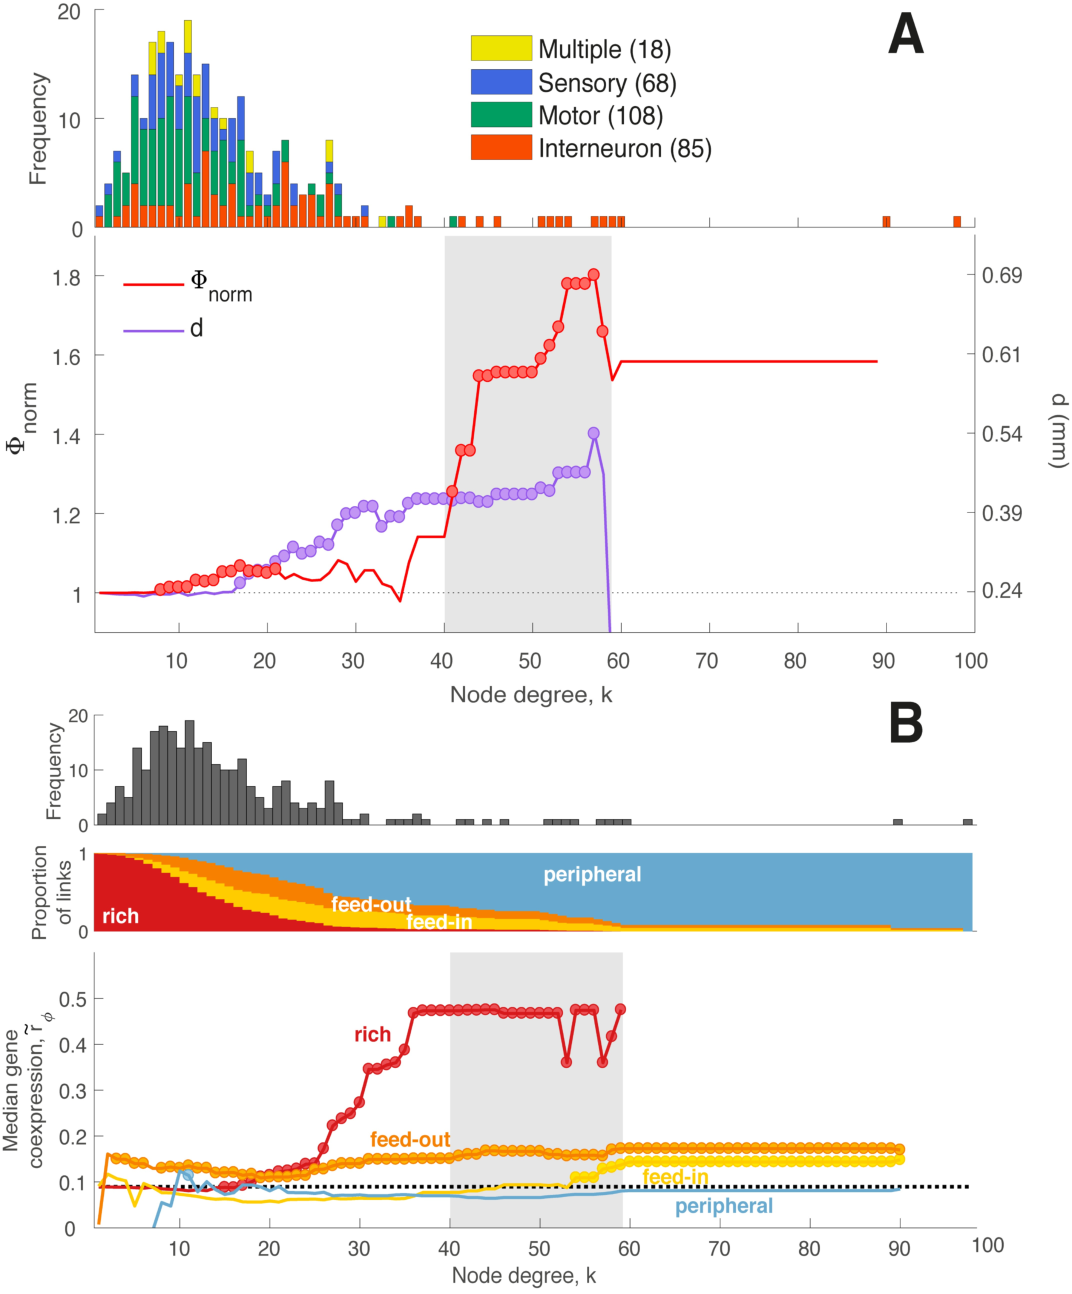
\includegraphics[width=0.6\textwidth]{Chapter2/Ch2S1fig.pdf}}
 \caption{{\bf Rich club organisation and correlated gene expression in synaptic connectivity matrix.}
(A) Rich-club organization of the synaptic \textit{C.elegans} connectome.
Top: Degree distribution of neurons, labelled to four categories: (i) interneuron (85 neurons, orange), (ii) motor (108 neurons, green), (iii) sensory (68 neurons, blue), or (iv) multiple assignments (18 neurons, yellow).
The distribution features an extended tail of high-degree neurons. Bottom: Normalized rich club coefficient, $\Phi_\mathrm{norm}$ (red), as a function of the degree, $k$, at which hubs are defined (as neurons with degree $>k$).
Also shown is the mean Euclidean separation distance, d (purple) between connected hub regions (across degree thresholds, k). $\Phi_\mathrm{norm} > 1$ indicates that hubs are more densely interconnected among each other than expected by chance, with red circles indicating values of $\Phi_\mathrm{norm}$ that are significantly higher than an ensemble of 1000 degree-matched null networks ($p < 0.05$).
Purple circles indicate where the Euclidean distance between connected pairs of hubs is significantly greater than the Euclidean distance for all other pairs of connected regions (right-tailed Welch's t-test, $p < 0.05$).
(B) Top: Degree distribution, $k$, of the synaptic \textit{C.elegans}  connectome.
Middle: proportion of connections that are: `rich' (hub $\rightarrow$ hub, red), `feed-in' (nonhub $\rightarrow$ hub, yellow), `feed-out' (hub $\rightarrow$ nonhub, orange), or `peripheral' (nonhub $\rightarrow$ nonhub, blue) as a function of the degree threshold, $k$, used to define hubs.
Note that at high $k$ most neurons are labeled as nonhubs and hence the vast majority of connections are labeled `peripheral'.
Bottom: Median CGE, $\tilde{r}_\phi$, for each connection type as a function of $k$.
The median CGE across all network links is shown as a dotted black line; the topological rich-club regime (determined from the network topology, cf. A) is shaded gray.
Circles indicate a statistically significant increase in CGE in a given link type relative to the rest of the network (one-sided Wilcoxon rank-sum test, $p < 0.05$).}

\label{fig:Ch2S1_Fig}
\end{figure}

%% FIGURE S2
\begin{figure}[h!]
  \centering{\includegraphics[width=1\textwidth]{Chapter2/Ch2S2fig.pdf}}
 \caption{{\bf Dependence of correlated gene expression measures on the proportion of positive annotations.} We plot the mean value of each metric across 1000 different pairs of random, binary vectors of length 948, which vary only in their proportion of `1's (between 0--0.15; corresponding to a number of `1's ranging from 1 to 150).
This is repeated for:
(A) mean square contingency coefficient, $r_\phi$,
(B) Jaccard index,
(C) Yule's $Q$, and
(D) our developed positive match measure, $p_\mathrm{match}$, (see \ref{app:AppendixCh2_3}).
Any systematic trend in correlation values indicates a bias driven by the proportion of positive annotations for a pair of vectors, as is seen for the Jaccard index and Yule's $Q$.
By contrast, $r_\phi$, which is used through this work, and our probability-based measure, $p_\mathrm{match}$, used to motivate individual gene scoring for enrichment analysis, show no evidence of systematic bias (note the color axis scales)}.
\label{fig:Ch2S2_Fig}
\end{figure}


%% FIGURE S3
\begin{figure}[h!]
  \centering{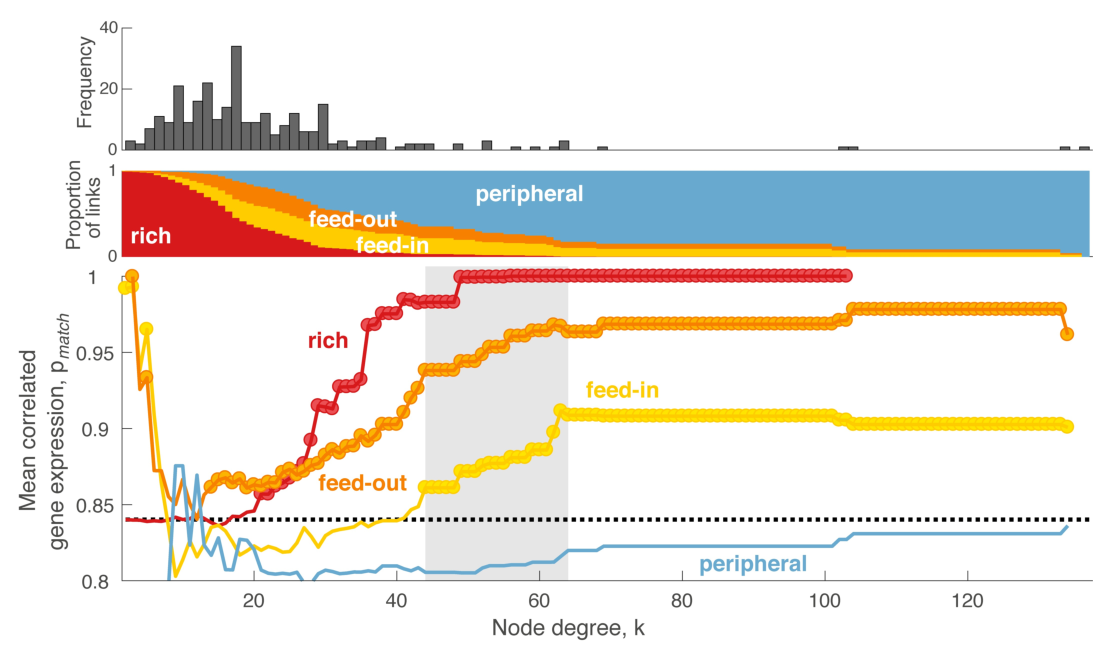
\includegraphics[width=1\textwidth]{Chapter2/Ch2S3fig.pdf}}
 \caption{{\bf Correlated gene expression measured using the positive matching probability index.} The matching probability index, $p_\mathrm{match}$, as introduced in \ref{app:AppendixCh2_3}.
\emph{Top}: Degree distribution.
\emph{Middle}: Proportion of connections that are `rich' (hub$\rightarrow$hub, red), `feed-in' (nonhub$\rightarrow$hub, yellow), `feed-out' (hub$\rightarrow$nonhub, orange), and `peripheral' (nonhub$\rightarrow$nonhub, blue) as a function of the degree threshold, $k$, used to define hubs.
Note that at high $k$, most neurons are labeled as nonhubs, and hence the vast majority of connections are `peripheral'.
\emph{Bottom}: Mean CGE calculated using similarity index from only positive matches, $p_{match}$, for each connection type as a function of $k$.
The mean CGE across all network links shown as a dotted black line; the topological rich-club regime (determined from the network topology, Figure \ref{fig:Ch2Fig5}) is shaded gray.
Circles indicate a statistically significant increase in CGE in a given link type relative to the rest of the network (one-sided Welch's $t$ test; $p < 0.05$).}
\label{fig:Ch2S3_Fig}
\end{figure}



%% FIGURE S4
\begin{figure}[h!]
  \centering{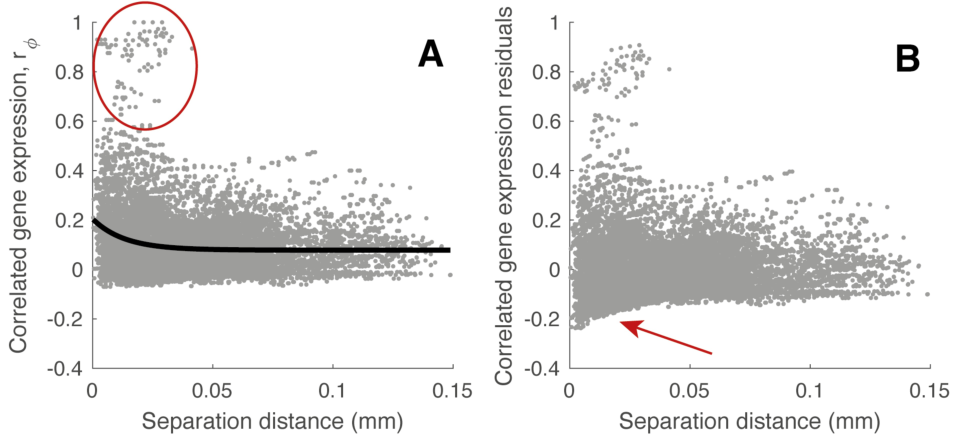
\includegraphics[width=1\textwidth]{Chapter2/Ch2S4fig.pdf}}
 \caption{{\bf Correcting for spatial effects in CGE data using a bulk exponential trend.}
  Here we consider correlated gene expression in the head, where the strongest spatial relationship exists (Figure \ref{fig:Ch2Fig4}. (A) CGE values, $r_\phi$, plotted as a function of Euclidean separation distance for all pairs of neurons within the head (gray dots), with a fitted exponential trend shown in black, $f(x) = A\exp(-\lambda x) + B$.
(B) Taking residuals from this trend does not adequately correct the spatial trend.
    Note the artifactual negative correlations indicated with an arrow.
    This indicates that the trend is not a bulk, isotropic effect, but may instead be driven primarily by a small number of neuron pairs with high $r_\phi$ at short distances ($\lessapprox 50\mu$m), indicated with a circle in (A).
For example, neuron pairs with $r_\phi > 0.8$, are all between the following classes of head neurons: CEP, IL1, OLQ, RMD, RME, RMF, SAAD, SAAV, SAB, SIA, SIB, SMB, SMD, URA, URY.}
\label{fig:Ch2S4_Fig}
\end{figure}


%% FIGURE S5
\begin{figure}[h!]
  \centering{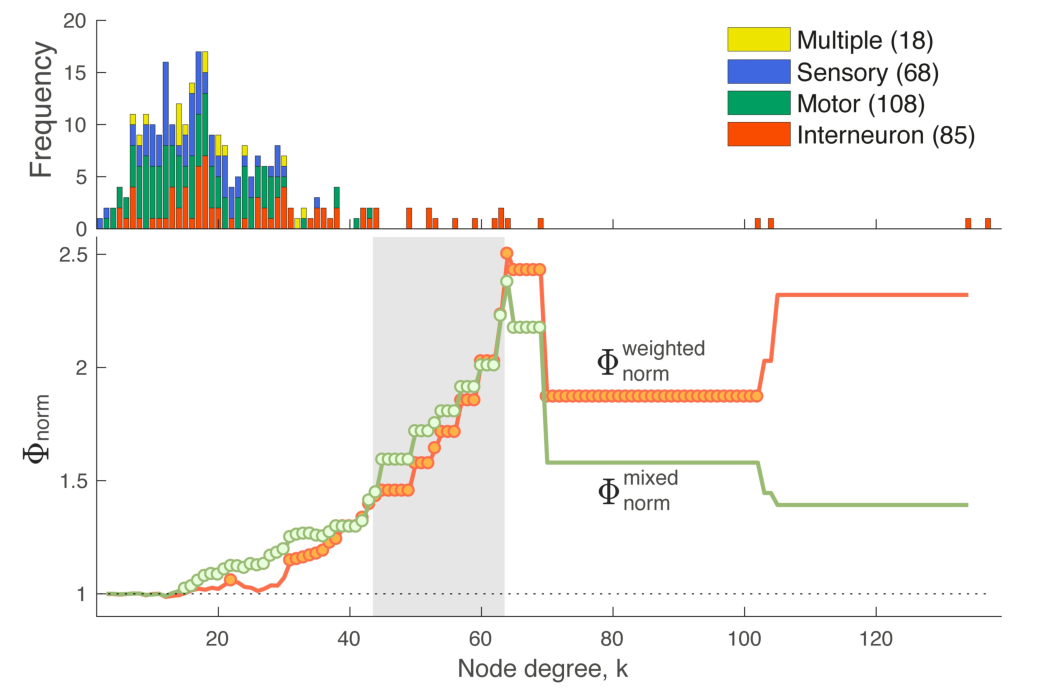
\includegraphics[width=1\textwidth]{Chapter2/Ch2S5fig.pdf}}
 \caption{{\bf Weighted and unweighted rich-club analyses yield similar results.}
   (A) Degree distribution of the \emph{C.elegans} connectome.
    Neurons are labeled to four types as in the legend.
    (B)
    Normalized weighted rich-club coefficient, $\Phi_\mathrm{norm}^\mathrm{weighted}$ (i.e., topology fixed and weights randomized in the null model, shown orange), and
    normalized mixed rich-club coefficient, $\Phi_\mathrm{norm}^\mathrm{mixed}$ (i.e., both topology and weights mixed in the null model, shown green) are plotted as a function of the degree, $k$, at which hubs are defined (as neurons with degree $>k$) \citep{Alstott2014}.
    Circles indicate values of $\Phi_\mathrm{norm}$ that are significantly higher than an ensemble of 1\,000 degree-matched null networks (Welch's $t$-test, $p < 0.05$).
    Compared to topological rich-club analysis presented in the main text, here the weights of the connections are also accounted for when calculating the rich club coefficient.
    In the case of the weighted rich-club coefficient, the topology for the null models was kept stable and only the weights of the connections randomized. Results presented here show that connections between higher degree nodes are stronger than expected by chance.
    On the other hand, in the mixed rich club coefficient both the topology and weights are randomized, therefore we see the combined effect of both types.
    Distinction between the different null models is discussed in detail in \citep{Alstott2014}.
    These results show that connections between high degree nodes are both denser and stronger than expected by chance.}
\label{fig:Ch2S5_Fig}
\end{figure}


\begin{figure}[h!]
  \centering{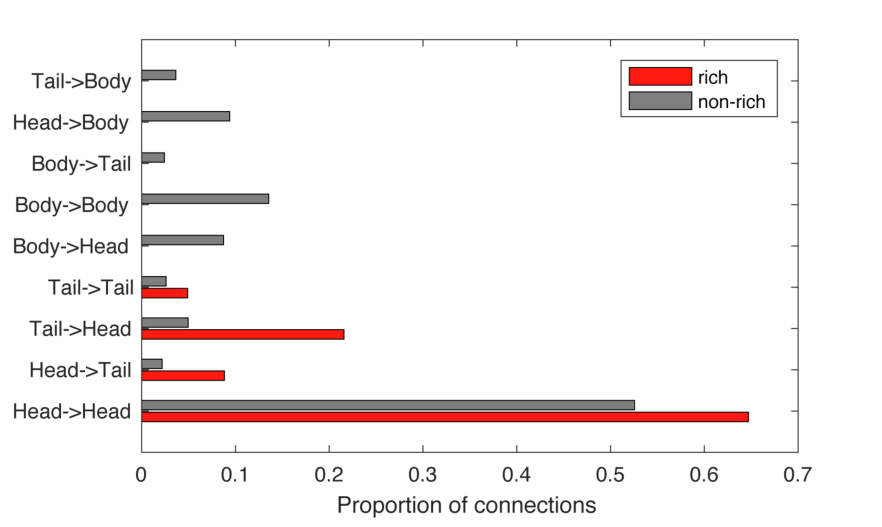
\includegraphics[width=1\textwidth]{Chapter2/Ch2S6fig.pdf}}
 \caption{{\bf Rich and non-rich connections in the \emph{C.elegans} connectome, categorized by the  anatomical location of the source and target neurons.}
   Hub-hub connections (`rich') are shown red, and all other connections (`non-rich', i.e., feeder and peripheral) are shown gray, where hubs are defined as neurons with degree, $k > 44$.
Anatomical locations are labeled as `head', `body', and `tail', and each connection is labeled according to its source and target neurons, listed on the vertical axis in the form `Source-Target'.
The plot shows that the increased separation distance between connected hubs relative to other types of connected neurons is driven by a relative increase in long-range connections between the head and tail.}
\label{fig:Ch2S6_Fig}
\end{figure}

\begin{figure}[h!]
  \centering{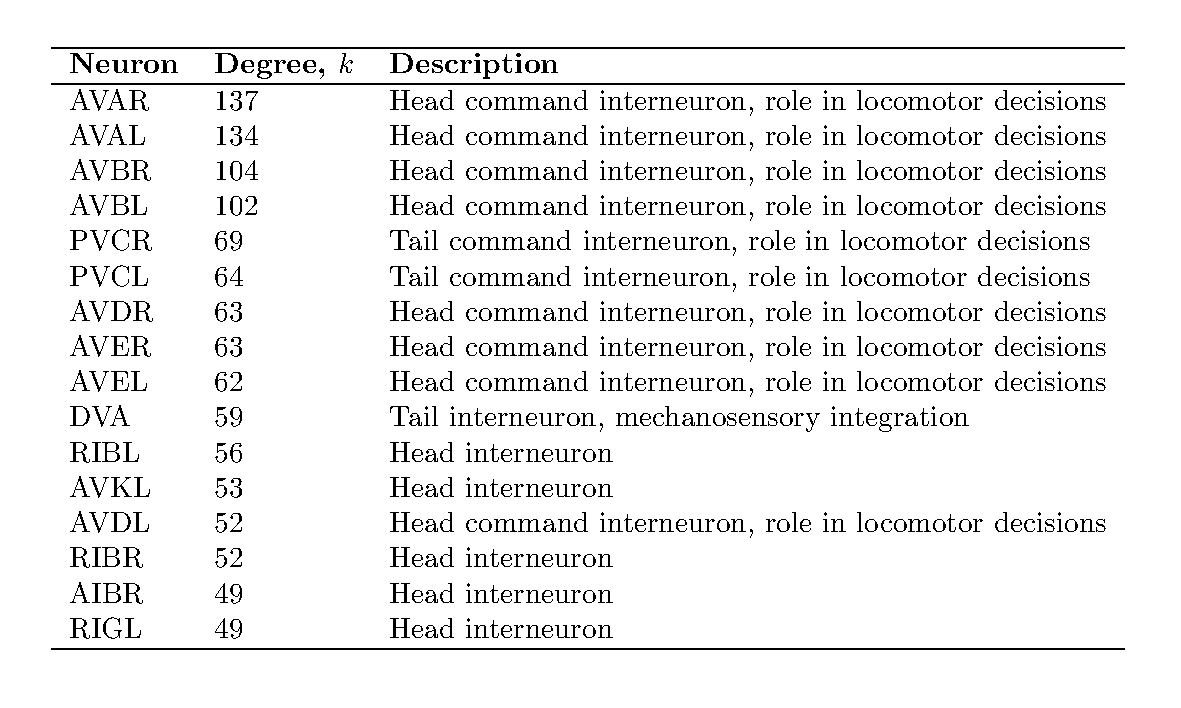
\includegraphics[width=1\textwidth]{Chapter2/Ch2S1Tab.pdf}}
   \caption{{\bf Hub neurons of the \textit{C.elegans} connectome.} Hubs are defined as neurons with degree $k > 44$. For each hub, we list (i) the neuron name, (ii) its degree, $k$, (iii) location (`head', `body', or `tail'), and function based on information presented in the wormatlas website \url{http://www.wormatlas.org/}.
Neurons are sorted (descending) by degree.}
\label{tab:HubList}
\end{figure}

\begin{figure}[h!]
  \centering{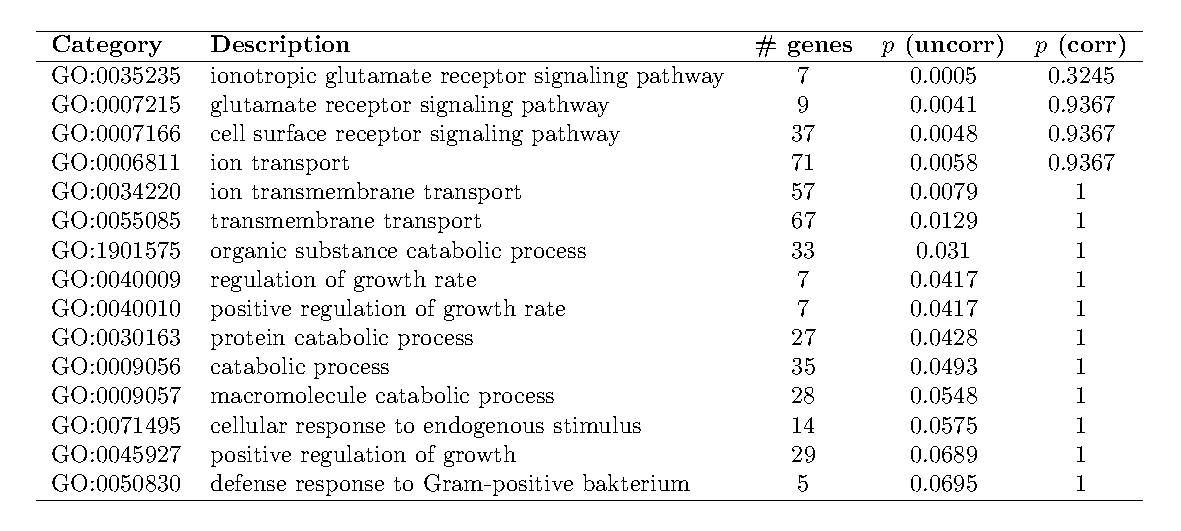
\includegraphics[width=1\textwidth]{Chapter2/Ch2S2Tab.pdf}}
   \caption{{\bf Enrichment results for connected \textit{vs} unconnected neurons.} Top 15 biological process GO categories enriched in genes with the highest mean increase in CGE for connected neurons compared to unconnected neurons.
Categories are sorted by $p$-value (ascending).}
\label{tab:enrichmentCON}
\end{figure}

\begin{figure}[h!]
  \centering{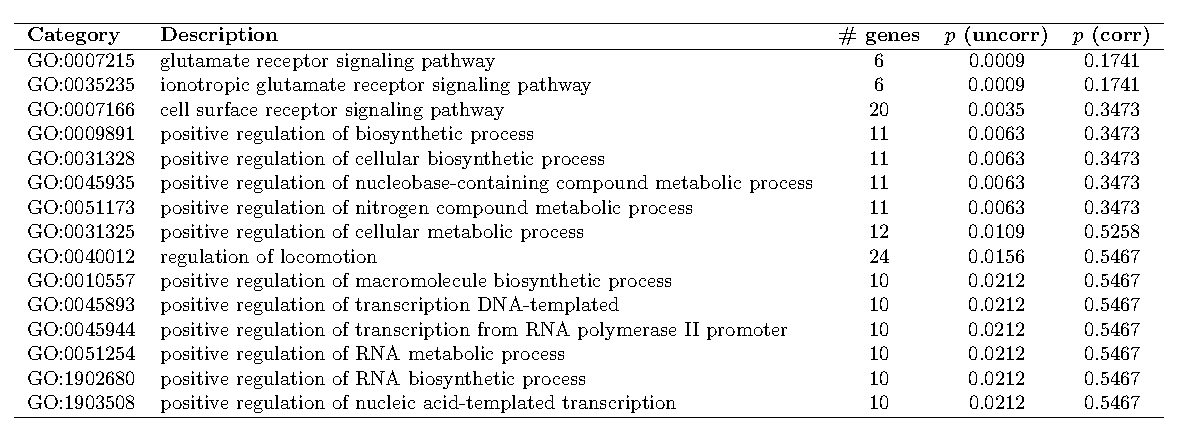
\includegraphics[width=1\textwidth]{Chapter2/Ch2S3Tab.pdf}}
   \caption{{\bf Enrichment results for links involving hubs.} Top 15 biological process GO categories enriched in genes with the highest increase in CGE for connections involving hub neurons (i.e., rich, feed-in and feed-out connections) compared to connections between nonhub neurons (i.e., in peripheral connections).
Categories are sorted by $p$-value (ascending).}
\label{tab:enrichmentRICH}
\end{figure}

\paragraph*{S1 File.}
\label{file:geneList}
{\bf Genes controbuting towards increased CGE.}
A list of genes that contributed towards the (i) increased CGE in connected compared to unconnected pairs of neurons, and (ii) increased CGE in rich and feeder compared to peripheral connections.
